\documentclass[a4paper]{article}
%\usepackage{vntex}
%\usepackage[english,vietnam]{babel}
%\usepackage[utf8]{inputenc}

%\usepackage[utf8]{inputenc}
%\usepackage[francais]{babel}
\usepackage{a4wide,amssymb,epsfig,latexsym,multicol,array,hhline,fancyhdr}

\usepackage{verbatim}
\usepackage{amsmath}
\usepackage{lastpage}
\usepackage[lined,boxed,commentsnumbered]{algorithm2e}
\usepackage{enumerate}
\usepackage{color}
\usepackage{graphicx}							% Standard graphics package
\usepackage{array}
\usepackage{tabularx, caption}
\usepackage{multirow}
\usepackage{multicol}
\usepackage{rotating}
\usepackage{graphics}
\usepackage{geometry}
\usepackage{setspace}
\usepackage{epsfig}
\usepackage{tikz}
\usepackage{ltablex}
\usepackage{enumitem}
\usetikzlibrary{arrows,snakes,backgrounds}
\usepackage{hyperref}
\usepackage{color, colortbl}
\hypersetup{urlcolor=blue,linkcolor=black,citecolor=black,colorlinks=true} 
%\usepackage{pstcol} 								% PSTricks with the standard color package


%\usepackage{fancyhdr}
\setlength{\headheight}{40pt}
\pagestyle{fancy}
\fancyhead{} % clear all header fields
\fancyhead[L]{
 \begin{tabular}{rl}
    \begin{picture}(25,15)(0,0)
    \put(0,-8){
\includegraphics[width=8mm, height=8mm]{hcmut.png}}
    %\put(0,-8){\epsfig{width=10mm,figure=hcmut.eps}}
   \end{picture}&
	%
\includegraphics[width=8mm, height=8mm]{hcmut.png} & %
	\begin{tabular}{l}
		\textbf{\bf \ttfamily Ho Chi Minh University of Technology}\\
		\textbf{\bf \ttfamily Faculty of Computer Science and Engineering}
	\end{tabular} 	
 \end{tabular}
}
\fancyhead[R]{
	\begin{tabular}{l}
		\tiny \bf \\
		\tiny \bf 
	\end{tabular}  }
\fancyfoot{} % clear all footer fields
\fancyfoot[L]{\scriptsize \ttfamily Operating System Lab}
\fancyfoot[R]{\scriptsize \ttfamily Page {\thepage}/\pageref{LastPage}}
\renewcommand{\headrulewidth}{0.3pt}
\renewcommand{\footrulewidth}{0.3pt}


%%%
\setcounter{secnumdepth}{4}
\setcounter{tocdepth}{3}
\makeatletter
\newcounter {subsubsubsection}[subsubsection]
\renewcommand\thesubsubsubsection{\thesubsubsection .\@alph\c@subsubsubsection}
\newcommand\subsubsubsection{\@startsection{subsubsubsection}{4}{\z@}%
                                     {-3.25ex\@plus -1ex \@minus -.2ex}%
                                     {1.5ex \@plus .2ex}%
                                     {\normalfont\normalsize\bfseries}}
\newcommand*\l@subsubsubsection{\@dottedtocline{3}{10.0em}{4.1em}}
\newcommand*{\subsubsubsectionmark}[1]{}
\makeatother

\definecolor{Gray}{gray}{0.9}

\begin{document}

\begin{titlepage}
\begin{center}
HO CHI MINH UNIVERSITY OF TECHNOLOGY \\
FACULTY OF COMPUTER SCIENCE AND ENGINEERING 
\end{center}

\vspace{1cm}

\begin{figure}[h!]
\begin{center}

\includegraphics[width=3cm]{hcmut.png}
\end{center}
\end{figure}

\vspace{1cm}


\begin{center}
\begin{tabular}{c}
\multicolumn{1}{c}{\textbf{{\Large OPERATING SYSTEM LAB (CO2018)}}}\\
~~\\
\hline
\\
\textbf{{\Huge LAB 6 : SYNCHRONIZATION}}\\
%\textbf{{\Large (Submission 1)}}\\
\\
\hline
\end{tabular}
\end{center}

\vspace{3cm}

\begin{table}[h]
\begin{tabular}{rrl}
\hspace{5 cm} & Teacher: & Tran Truong Tuan Phat\\
& Student: & Thai Phuc Hiep - 1812227 \\
\end{tabular}
\end{table}

\vspace{4.7cm}

\begin{center}
{\footnotesize HO CHI MINH CITY, May 2020}
\end{center}
\end{titlepage}


%\thispagestyle{empty}

\newpage
\tableofcontents
\newpage

\section{PROBLEM 1 :}
We assume that :
\begin{itemize}
\item balance = 20.000.000 VND 
\item The husband calls function : \texttt{withdraw(5.000.000)}
\item The wife calls function : \texttt{deposit(10.000.000)}
\end{itemize}
All possible outcomes we could get :

\begin{itemize}

\item \texttt{withdraw()} is executed \textbf{before} \texttt{deposit()} :
\begin{itemize}
\item \texttt{withdraw(5.000.000)} $\Rightarrow$ balance = 20.000.000 - 5.000.000 = 15.000.000 (VND) 
\item \texttt{deposit(10.000.000)} $\Rightarrow$ balance = 15.000.000 + 10.000.000 = 25.000.000 (VND)
\end{itemize}

\item \texttt{withdraw()} is executed \textbf{after} \texttt{deposit()} :
\begin{itemize}
\item \texttt{deposit(10.000.000)} $\Rightarrow$ balance = 20.000.000 + 10.000.000 = 30.000.000 (VND) 
\item \texttt{withdraw(5.000.000)} $\Rightarrow$ balance = 30.000.000 - 5.000.000 = 25.000.000 (VND)
\end{itemize}
	
\item \texttt{withdraw()} and \texttt{deposit()} are executed \textbf{concurrently} :
\begin{itemize}
\item \texttt{withdraw(5.000.000)} $\Rightarrow$ balance = 20.000.000 - 5.000.000 = 15.000.000 (VND) 
\item Concurrently, \texttt{deposit(10.000.000)} $\Rightarrow$ balance = 20.000.000 + 10.000.000 = 30.000.000 (VND)
\end{itemize}
\end{itemize}
As we can see, the third case show the unexpected result, since \texttt{withdraw()} function and \texttt{deposit()} function change the balance value at the same time. \\
\\
\textbf{Solution} : Use mutex or semaphore. 

\section{PROBLEM 2 :}
Comparison Condition :
\begin{itemize}
\item Number of threads = 1000
\item Number of points = 1000000
\end{itemize}
Here is the result :
\begin{itemize}
\item \texttt{pi\textunderscore mutex} : 0.051486 s
\item \texttt{pi\textunderscore multi-thread} : 0.050707 s
\end{itemize}
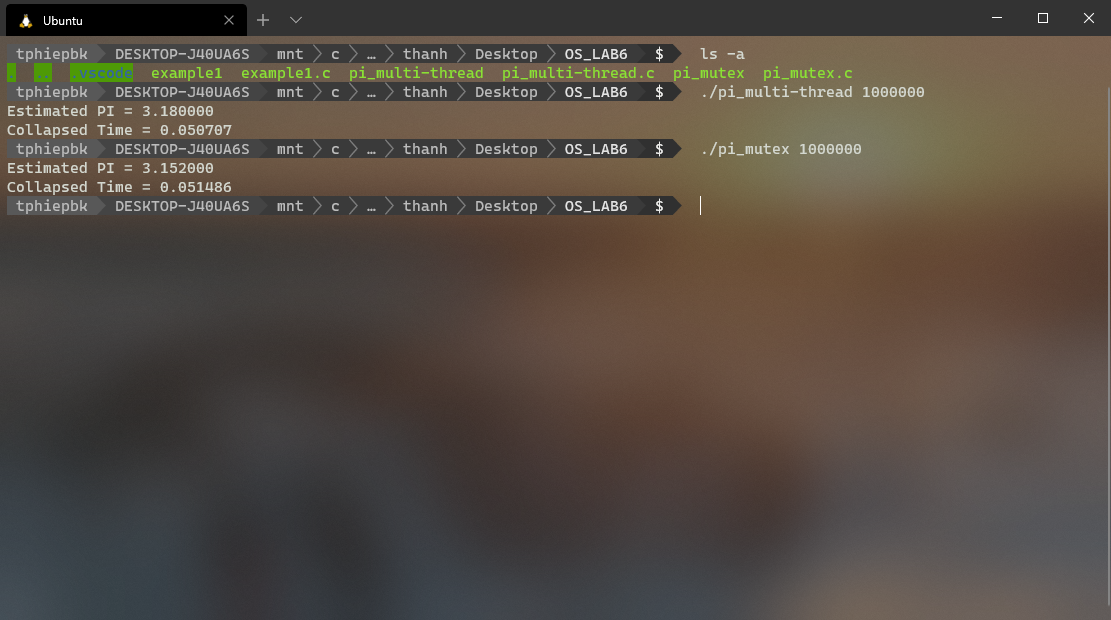
\includegraphics[scale=0.5]{compare.png} \\
\\
So the mutex lock approach is slower than the multi-thread approach.
\end{document}

